\documentclass[11pt,a4paper,titlepage]{article}
\usepackage{ifpdf}
\usepackage[utf8]{inputenc}
\usepackage[francais]{babel}
\usepackage[T1]{fontenc}
%\usepackage[top=3cm,right=3.5cm,bottom=3cm,left=3.5cm]{geometry}
\usepackage{graphicx}

\newcommand{\HRule}{\rule{\linewidth}{0.5mm}} %Pour mettre dans la title page
\parindent 1.0cm
\title{Intelligence Artificielle : Atari Go}
\author{Julien \textsc{Durillon} \and Clotilde \textsc{Massot}}
\date{\today}

%Partie pdf
\ifpdf
\pdfinfo {
	/Author (Julien Durillon - Clotilde Massot)
	/Title (Intelligence Artificielle : Atari Go)
	/Subject (Intelligence Artificielle : Atari Go)
	/Keywords (IA, go, alma)
	/CreationDate (D:20100219175732)
}
\fi
%Fin partie pdf


\begin{document}
%	\maketitle
	\begin{titlepage}

\begin{center}


% Upper part of the page

\includegraphics[scale=1.00]{./logo_fac.png}
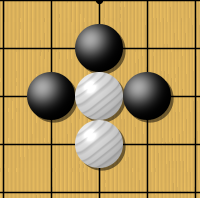
\includegraphics[scale=0.5]{./logogo.png}\\[1cm]

\textsc{\LARGE Intelligence artificielle}\\[1.5cm]

\textsc{\Large Projet TP : Atari Go}\\[0.5cm]


% Title
\HRule \\[0.4cm]
{ \huge \bfseries Étude du jeu et des possibilités d'heuristique}\\[0.4cm]

\HRule \\[1.5cm]

% Author and supervisor
\begin{minipage}{0.4\textwidth}
\begin{flushleft} \large
\emph{Auteurs :}\\[0.2cm]
\end{flushleft}
\end{minipage}

\begin{minipage}{0.5\textwidth}
\begin{flushright} \large
Clotilde \textsc{Massot}\\
Julien \textsc{Durillon}
\end{flushright}
\end{minipage}

\vfill

% Bottom of the page
{\large \today}

\end{center}
\end{titlepage}


	\tableofcontents
	\clearpage

	\abstract{Ce document explique l'étude du cas de l'atari go dans le cadre du projet d'IA du master 1 ALMA 2010. Y sera utilisé la méthode Alpha-Beta pour gérer l'arbre des possibles.}

	\section*{Introduction}
		Le projet demandé dans ce module d'intelligence artificielle est de développer un programme capable de jouer à l'atari go. Ce jeu est une modification du jeu de go traditionnel, jeu inventé en chine médiévale. La version Atari go que nous allons traiter se joue sur un goban plus petit --- d'une taille de 9x9. Le but est d'être le premier à prendre des pierres à l'adversaire. Quand une prise a été effectuée, le jeu est fini. Nous parlerons de pierres ou groupes \emph{adverses} pour désigner les pierres et groupes de l'adversaire, et \emph{alliés} pour désigner les nôtres --- i.e. ceux joués par le programme.

		Nous commencerons par expliciter notre démarche de développement, puis nous continuerons par décrire le cheminement de notre recherche sur les heuristiques, et finirons en présentant l'implémentation de l'algorithme Alpha-Beta, ainsi qu'une éventuelle interface, et les améliorations apportées et pouvant l'être.

	\section{Mise en place du projet}
		\subsection{Environnement}
		\subsection{Partage du travail}
			L'étude est faite en binôme, et les classes de description du goban ont été faites de la même façon. Le travail est ensuite partagé comme ceci : Clotilde Massot implémente dans un premier temps l'algorithme Alpha-Beta, tandis que Julien Durillon prépare la partie heuristique --- calcul de groupes de pierres\dots --- % Expliquer l'interface


	\section{Heuristique}

		\subsection{Un premier jet}
			Un premier indice utilisé pour déterminer l'état d'un jeu est d'identifier les groupes de pierres, et calculer leurs libertés, et noter les différents groupes en fonction de ce critère. On s'intéresse au groupe qui a le moins de libertés. Si un groupe ami a 0 liberté, on fixe le score à $-\infty$ (en java, on prendra $-MAX\_LONG$). À l'inverse, si un groupe adverse a 0 libertés, on fixe le score à $+\infty$.

			Cette méthode va entraîner une tendance à construire des longues chaînes. Il faut donc chercher une heuristique plus fine.

		\subsection{Affiner les cas gagnant ou perdant}
			Un cas gagnant --- resp. perdant --- est à première vue un cas où un groupe adverse --- resp. allié --- n'a plus aucune liberté. Mais il existe d'autres cas où un groupe est dit \emph{mort}, c'est-à-dire qu'il ne peut plus sortir vivant. Un des cas les plus évidents est le cas (c.f. figure \ref{groupemort}) où il ne reste plus qu'une libertée, et que l'adversaire est déjà autour de cette liberté.

			\begin{figure}[bht]
			\begin{center}
			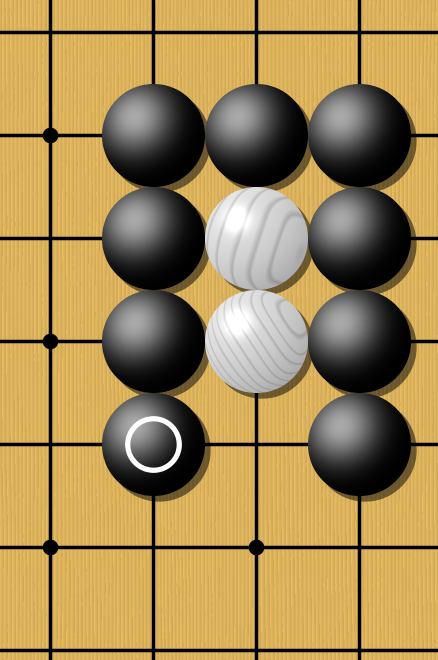
\includegraphics[width=0.4\textwidth]{groupemort.png}
			\end{center}
			\caption{Le groupe blanc est mort}
			\label{groupemort}
			\end{figure}

		\subsection{Les yeux}
			Au go, un groupe ayant deux yeux est dit imprenable --- cf. figure \ref{deuxyeux} . Un amélioration de la fonction présentée ci-dessus peut être de détecter de telles dispositions ; en effet, un groupe ayant deux yeux d'une case chacun peut n'avoir que 2 libertés tout en restant imprenable. On noterait alors mieux de tels groupes, et on aurait pas à s'en «~soucier~». Pour détecter de tels yeux, il «~suffit~» de chercher des libertés entourées uniquement du bord ou de pierres du groupe étudié. Nous pouvons assez facilement détecter des cas simples d'yeux.

			\begin{figure}[bht]
			\begin{center}
			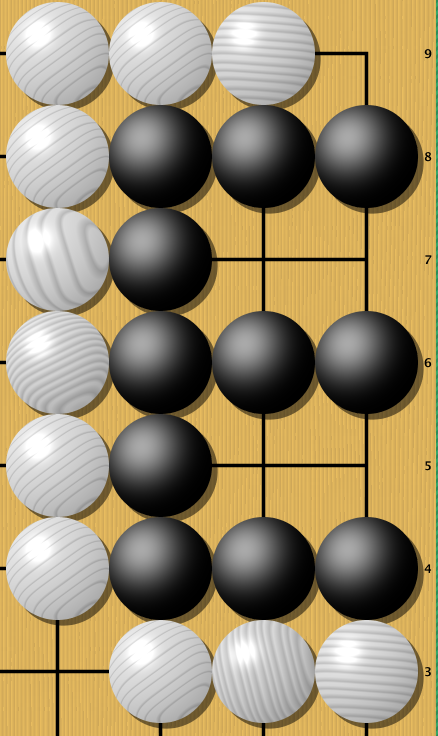
\includegraphics[width=0.4\textwidth]{deuxyeux.png}
			\end{center}
			\caption{Le groupe noir a deux yeux}
			\label{deuxyeux}
			\end{figure}

		\subsection{Les sauts}

			Une des formes intéressantes est le coup en diagonale ou \emph{kosumi} --- cf. figure \ref{kosumi}. Ce coup fait un lien entre les deux pierre qui n'existe pas encore, mais qui ne peut être coupé en un seul coup. Dans la figure \ref{kosumi}, si blanc joue dans le cercle, noir connecte dans le triangle, et vice-versa.

			\begin{figure}[bht]
			\begin{center}
			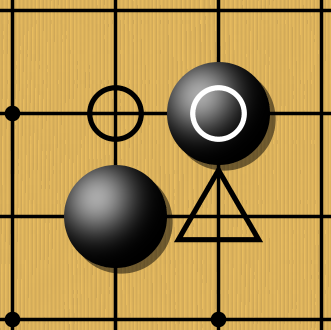
\includegraphics[width=0.3\textwidth]{kosumi.png}
			\end{center}
			\caption{Kosumi}
			\label{kosumi}
			\end{figure}

	\section{Algorithme Alpha-Beta}

		\subsection{Base}

		\subsection{Amélioration possible de l'algorithme}
			Pour améliorer cet algorithme, on peut définir plusieurs fonctions d'analyse du jeu, correspondant à plusieurs cas : Une fonction pour un cas neutre : ni plutôt avantageux, ni plutôt mauvais, une fonction pour un cas mauvais (où on est en train de perdre), et une fonction pour un cas où on est en train de gagner.
\end{document}
